% Options for packages loaded elsewhere
\PassOptionsToPackage{unicode}{hyperref}
\PassOptionsToPackage{hyphens}{url}
%
\documentclass[
  10pt,
  ignorenonframetext,
  aspectratio=1612]{beamer}
\usepackage{pgfpages}
\setbeamertemplate{caption}[numbered]
\setbeamertemplate{caption label separator}{: }
\setbeamercolor{caption name}{fg=normal text.fg}
\beamertemplatenavigationsymbolsempty
% Prevent slide breaks in the middle of a paragraph
\widowpenalties 1 10000
\raggedbottom
\setbeamertemplate{part page}{
  \centering
  \begin{beamercolorbox}[sep=16pt,center]{part title}
    \usebeamerfont{part title}\insertpart\par
  \end{beamercolorbox}
}
\setbeamertemplate{section page}{
  \centering
  \begin{beamercolorbox}[sep=12pt,center]{part title}
    \usebeamerfont{section title}\insertsection\par
  \end{beamercolorbox}
}
\setbeamertemplate{subsection page}{
  \centering
  \begin{beamercolorbox}[sep=8pt,center]{part title}
    \usebeamerfont{subsection title}\insertsubsection\par
  \end{beamercolorbox}
}
\AtBeginPart{
  \frame{\partpage}
}
\AtBeginSection{
  \ifbibliography
  \else
    \frame{\sectionpage}
  \fi
}
\AtBeginSubsection{
  \frame{\subsectionpage}
}
\usepackage{amsmath,amssymb}
\usepackage{iftex}
\ifPDFTeX
  \usepackage[T1]{fontenc}
  \usepackage[utf8]{inputenc}
  \usepackage{textcomp} % provide euro and other symbols
\else % if luatex or xetex
  \usepackage{unicode-math} % this also loads fontspec
  \defaultfontfeatures{Scale=MatchLowercase}
  \defaultfontfeatures[\rmfamily]{Ligatures=TeX,Scale=1}
\fi
\usepackage{lmodern}
\usetheme[]{Warsaw}
\ifPDFTeX\else
  % xetex/luatex font selection
\fi
% Use upquote if available, for straight quotes in verbatim environments
\IfFileExists{upquote.sty}{\usepackage{upquote}}{}
\IfFileExists{microtype.sty}{% use microtype if available
  \usepackage[]{microtype}
  \UseMicrotypeSet[protrusion]{basicmath} % disable protrusion for tt fonts
}{}
\makeatletter
\@ifundefined{KOMAClassName}{% if non-KOMA class
  \IfFileExists{parskip.sty}{%
    \usepackage{parskip}
  }{% else
    \setlength{\parindent}{0pt}
    \setlength{\parskip}{6pt plus 2pt minus 1pt}}
}{% if KOMA class
  \KOMAoptions{parskip=half}}
\makeatother
\usepackage{xcolor}
\newif\ifbibliography
\usepackage{color}
\usepackage{fancyvrb}
\newcommand{\VerbBar}{|}
\newcommand{\VERB}{\Verb[commandchars=\\\{\}]}
\DefineVerbatimEnvironment{Highlighting}{Verbatim}{commandchars=\\\{\}}
% Add ',fontsize=\small' for more characters per line
\usepackage{framed}
\definecolor{shadecolor}{RGB}{248,248,248}
\newenvironment{Shaded}{\begin{snugshade}}{\end{snugshade}}
\newcommand{\AlertTok}[1]{\textcolor[rgb]{0.94,0.16,0.16}{#1}}
\newcommand{\AnnotationTok}[1]{\textcolor[rgb]{0.56,0.35,0.01}{\textbf{\textit{#1}}}}
\newcommand{\AttributeTok}[1]{\textcolor[rgb]{0.13,0.29,0.53}{#1}}
\newcommand{\BaseNTok}[1]{\textcolor[rgb]{0.00,0.00,0.81}{#1}}
\newcommand{\BuiltInTok}[1]{#1}
\newcommand{\CharTok}[1]{\textcolor[rgb]{0.31,0.60,0.02}{#1}}
\newcommand{\CommentTok}[1]{\textcolor[rgb]{0.56,0.35,0.01}{\textit{#1}}}
\newcommand{\CommentVarTok}[1]{\textcolor[rgb]{0.56,0.35,0.01}{\textbf{\textit{#1}}}}
\newcommand{\ConstantTok}[1]{\textcolor[rgb]{0.56,0.35,0.01}{#1}}
\newcommand{\ControlFlowTok}[1]{\textcolor[rgb]{0.13,0.29,0.53}{\textbf{#1}}}
\newcommand{\DataTypeTok}[1]{\textcolor[rgb]{0.13,0.29,0.53}{#1}}
\newcommand{\DecValTok}[1]{\textcolor[rgb]{0.00,0.00,0.81}{#1}}
\newcommand{\DocumentationTok}[1]{\textcolor[rgb]{0.56,0.35,0.01}{\textbf{\textit{#1}}}}
\newcommand{\ErrorTok}[1]{\textcolor[rgb]{0.64,0.00,0.00}{\textbf{#1}}}
\newcommand{\ExtensionTok}[1]{#1}
\newcommand{\FloatTok}[1]{\textcolor[rgb]{0.00,0.00,0.81}{#1}}
\newcommand{\FunctionTok}[1]{\textcolor[rgb]{0.13,0.29,0.53}{\textbf{#1}}}
\newcommand{\ImportTok}[1]{#1}
\newcommand{\InformationTok}[1]{\textcolor[rgb]{0.56,0.35,0.01}{\textbf{\textit{#1}}}}
\newcommand{\KeywordTok}[1]{\textcolor[rgb]{0.13,0.29,0.53}{\textbf{#1}}}
\newcommand{\NormalTok}[1]{#1}
\newcommand{\OperatorTok}[1]{\textcolor[rgb]{0.81,0.36,0.00}{\textbf{#1}}}
\newcommand{\OtherTok}[1]{\textcolor[rgb]{0.56,0.35,0.01}{#1}}
\newcommand{\PreprocessorTok}[1]{\textcolor[rgb]{0.56,0.35,0.01}{\textit{#1}}}
\newcommand{\RegionMarkerTok}[1]{#1}
\newcommand{\SpecialCharTok}[1]{\textcolor[rgb]{0.81,0.36,0.00}{\textbf{#1}}}
\newcommand{\SpecialStringTok}[1]{\textcolor[rgb]{0.31,0.60,0.02}{#1}}
\newcommand{\StringTok}[1]{\textcolor[rgb]{0.31,0.60,0.02}{#1}}
\newcommand{\VariableTok}[1]{\textcolor[rgb]{0.00,0.00,0.00}{#1}}
\newcommand{\VerbatimStringTok}[1]{\textcolor[rgb]{0.31,0.60,0.02}{#1}}
\newcommand{\WarningTok}[1]{\textcolor[rgb]{0.56,0.35,0.01}{\textbf{\textit{#1}}}}
\usepackage{graphicx}
\makeatletter
\def\maxwidth{\ifdim\Gin@nat@width>\linewidth\linewidth\else\Gin@nat@width\fi}
\def\maxheight{\ifdim\Gin@nat@height>\textheight\textheight\else\Gin@nat@height\fi}
\makeatother
% Scale images if necessary, so that they will not overflow the page
% margins by default, and it is still possible to overwrite the defaults
% using explicit options in \includegraphics[width, height, ...]{}
\setkeys{Gin}{width=\maxwidth,height=\maxheight,keepaspectratio}
% Set default figure placement to htbp
\makeatletter
\def\fps@figure{htbp}
\makeatother
\setlength{\emergencystretch}{3em} % prevent overfull lines
\providecommand{\tightlist}{%
  \setlength{\itemsep}{0pt}\setlength{\parskip}{0pt}}
\setcounter{secnumdepth}{-\maxdimen} % remove section numbering
\ifLuaTeX
  \usepackage{selnolig}  % disable illegal ligatures
\fi
\usepackage{bookmark}
\IfFileExists{xurl.sty}{\usepackage{xurl}}{} % add URL line breaks if available
\urlstyle{same}
\hypersetup{
  pdftitle={Análisis Descriptivo De la Serie de Tiempo del Café},
  pdfauthor={Angel Granados, Wilson Jerez, Santiago Montejo},
  hidelinks,
  pdfcreator={LaTeX via pandoc}}

\title{Análisis Descriptivo De la Serie de Tiempo del Café}
\author{Angel Granados, Wilson Jerez, Santiago Montejo}
\date{Junio 2024}

\begin{document}
\frame{\titlepage}

\begin{frame}{Introducción}
\phantomsection\label{introducciuxf3n}
Nuestro objetivo en este análisis es determinar si los precios del café
a lo largo del tiempo son estacionarios o no, utilizando la prueba de
Dickey-Fuller. Para lograr esto, exploraremos los datos de precios del
café desde 1980 hasta 2023, prestando especial atención al
comportamiento en el año 2000. Identificaremos las bajas significativas
en los precios según los registros de la bolsa de valores y evaluaremos
la confiabilidad de la inversión en este sector. Esto lo haremos
analizando la mayor caída en los precios del café durante este período y
explorando las oportunidades que podrían surgir en futuras caídas.
\end{frame}

\begin{frame}{Temáticas}
\phantomsection\label{temuxe1ticas}
Utilizando conceptos estadísticos como las series de tiempo y la prueba
de Dickey-Fuller, derivada de la teoría de series de tiempo,
determinaremos si los precios del café son estacionarios. La hipótesis
nula \((H0)\) en la prueba de Dickey-Fuller será que los precios no son
estacionarios, mientras que la hipótesis alternativa \((H1)\) será que
los precios son estacionarios. Adicionalmente, evaluaremos la
estacionalidad presente en los datos, que se manifiesta en patrones
recurrentes a lo largo del tiempo.

A través de este análisis, plantearemos y probaremos la hipótesis nula
de no estacionariedad y confirmaremos la presencia de estacionalidad.
\end{frame}

\begin{frame}{Serie de Tiempo}
\phantomsection\label{serie-de-tiempo}
Una serie de tiempo es una secuencia de datos recolectados y ordenados
cronológicamente, generalmente a intervalos regulares, como diarios,
mensuales, trimestrales o anuales. Estas series se utilizan para
analizar cómo una variable cambia a lo largo del tiempo y son
fundamentales en campos como la economía, la meteorología, la
ingeniería, y muchas otras disciplinas.
\end{frame}

\begin{frame}{Conceptos Importantes}
\phantomsection\label{conceptos-importantes}
\begin{enumerate}

  \item Estacionariedad:
  
  \item Tendencia
  
  \item Estacionalidad
  
  \item Ruido
  
  \item Prueba de Dickey-Fuller
  
  \item Modelos ARIMA (Autoregressive Integrated Moving Average)
  
  


\end{enumerate}
\end{frame}

\begin{frame}{Descripcion de la Base de Datos}
\phantomsection\label{descripcion-de-la-base-de-datos}
La base de datos utilizada para este análisis contiene información sobre
los precios del café, obtenida del sitio web Investing. Los datos
abarcan el período comprendido entre los años 1980 y 2023. Son datos
diarios que no abordan los fines de semana (Sabado y Domingo) y se
consideran dos Variables que son el tiempo (Expresado en Dias, Meses y
años) y el precio promedio diario.
\end{frame}

\begin{frame}[fragile]{Descripcion de la Base de Datos}
\phantomsection\label{descripcion-de-la-base-de-datos-1}
\begin{verbatim}
## 'data.frame':    11152 obs. of  8 variables:
##  $ Fecha          : Date, format: "1979-12-27" "1979-12-28" ...
##  $ Último         : num  183 182 182 178 172 ...
##  $ Apertura       : num  188 183 182 182 176 ...
##  $ Máximo         : num  188 186 183 182 176 ...
##  $ Mínimo         : num  183 181 181 176 170 ...
##  $ Vol.           : chr  "" "" "" "1,14K" ...
##  $ X..var.        : chr  "-2,23%" "-0,90%" "0,12%" "-2,29%" ...
##  $ precio_promedio: num  186 183 182 179 174 ...
\end{verbatim}
\end{frame}

\begin{frame}{Descripcion de la Base de Datos}
\phantomsection\label{descripcion-de-la-base-de-datos-2}
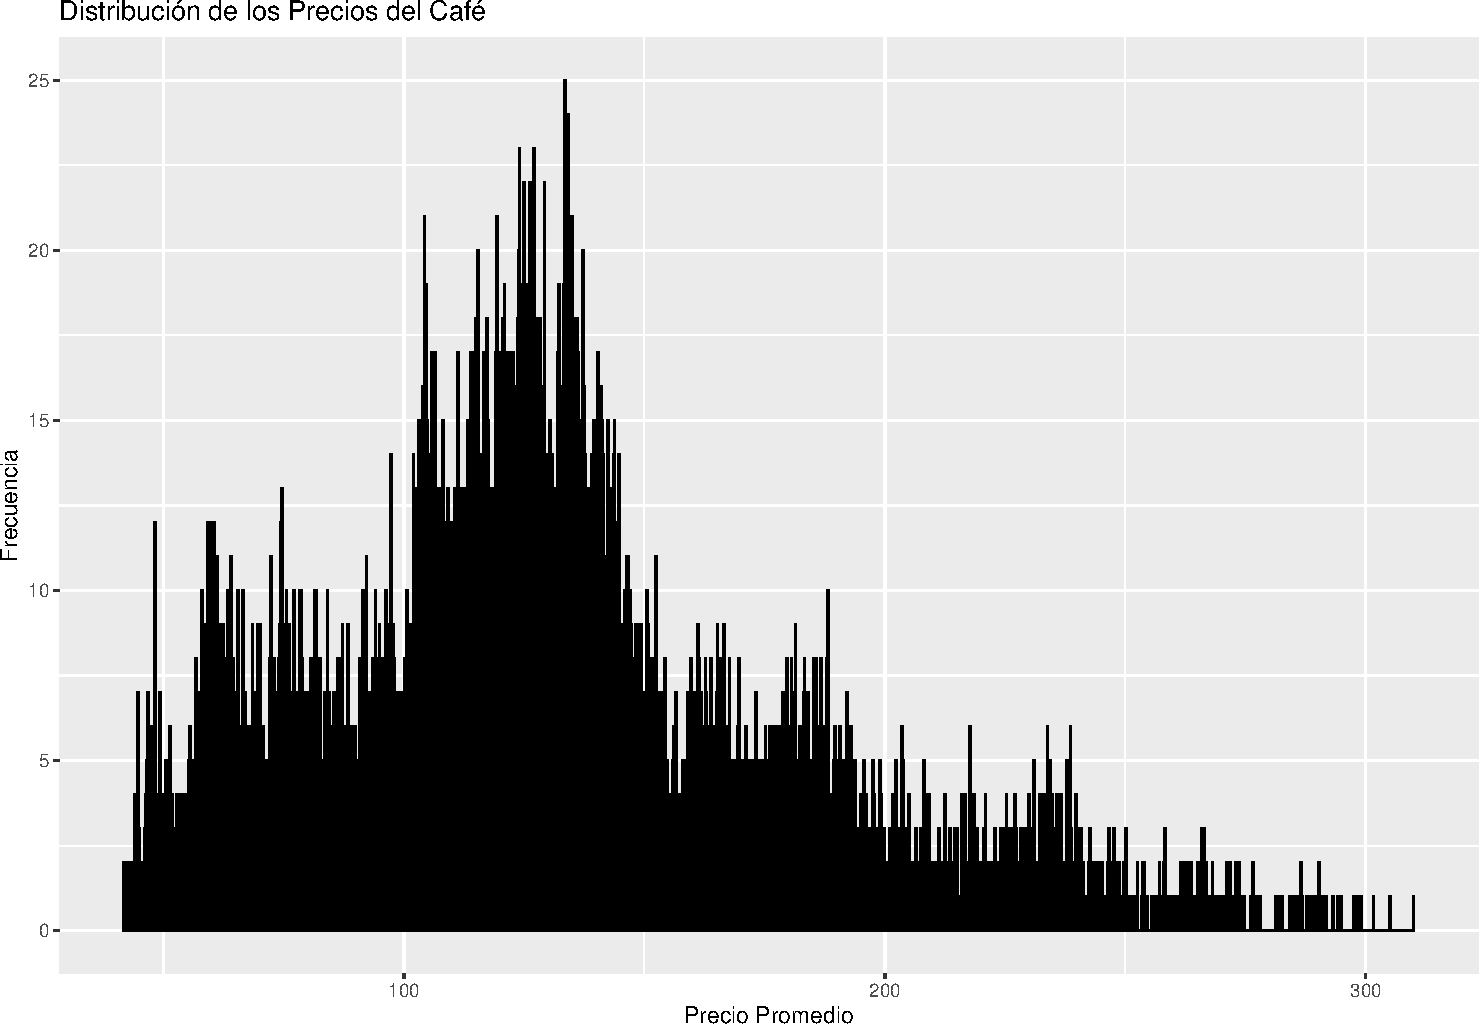
\includegraphics{Informe_files/figure-beamer/unnamed-chunk-2-1.pdf}
\end{frame}

\begin{frame}{Descripcion de la Base de Datos}
\phantomsection\label{descripcion-de-la-base-de-datos-3}
\begin{itemize}
\item
  Forma de la Distribución: Observando la forma del histograma, se puede
  identificar si los precios del café están distribuidos simétricamente,
  sesgados a la izquierda.
\item
  Centralidad: El centro de la distribución se puede estimar visualmente
  observando dónde se concentran los valores más frecuentes.
\item
  Dispersión: La dispersión de los datos puede ser evaluada observando
  la amplitud de los bins en el histograma y también considerando la
  varianza o el rango intercuartil (IQR). Un sesgo hacia la izquierda
  típicamente implica una menor dispersión hacia los valores más altos.
\end{itemize}
\end{frame}

\begin{frame}{Descripcion de la Base de Datos}
\phantomsection\label{descripcion-de-la-base-de-datos-4}
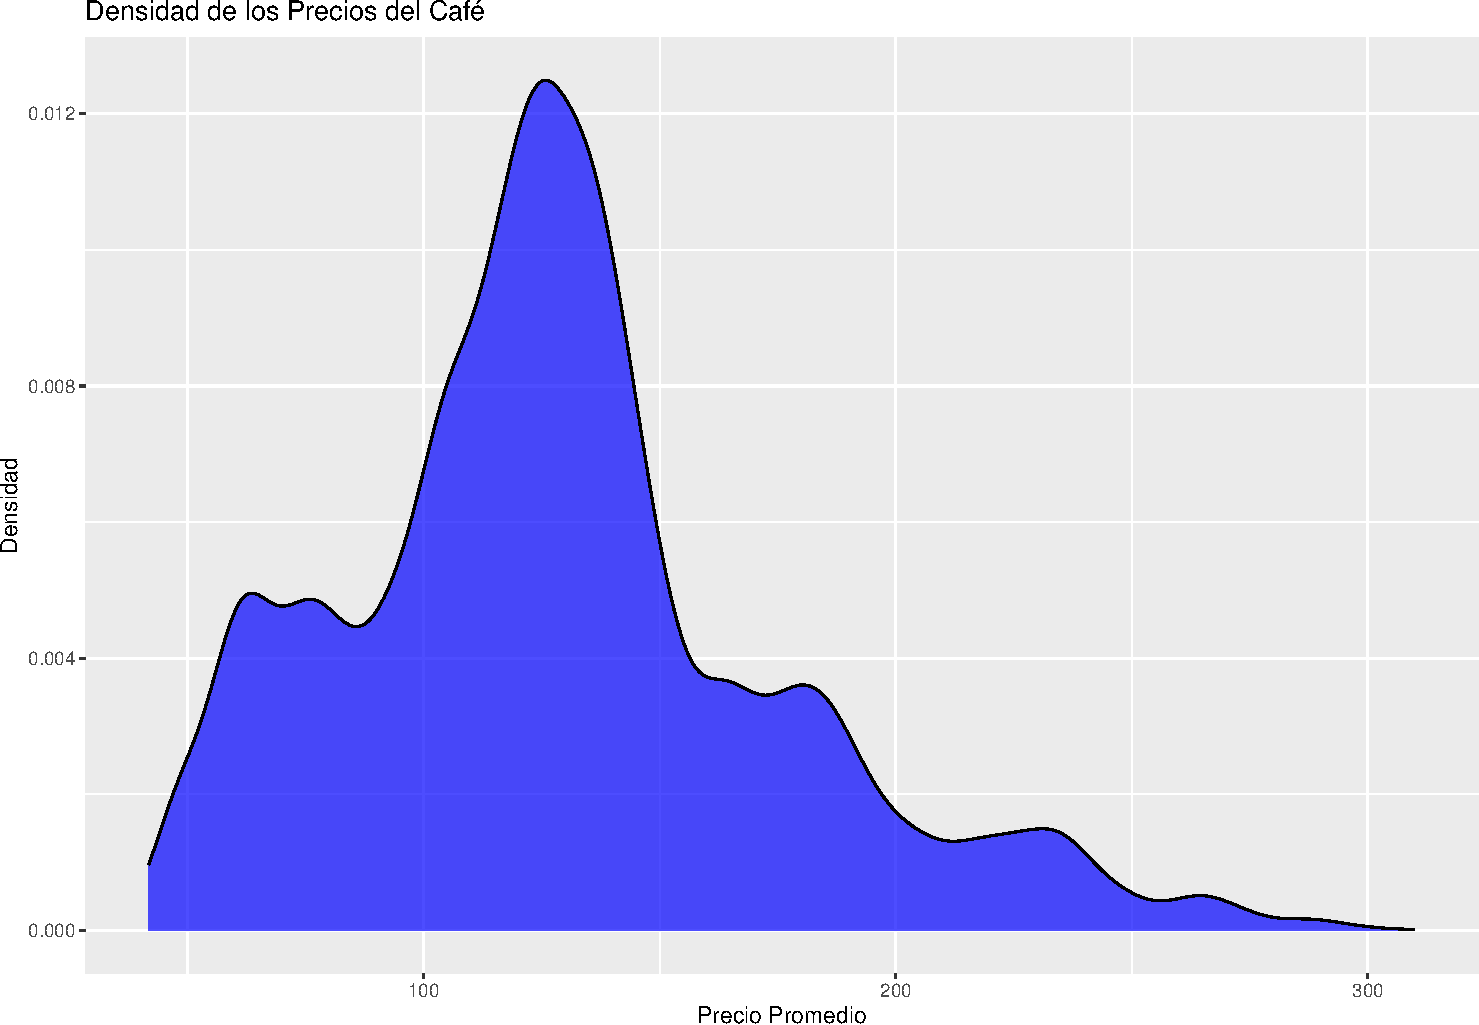
\includegraphics{Informe_files/figure-beamer/unnamed-chunk-3-1.pdf}
\end{frame}

\begin{frame}{Descripcion de la Base de Datos}
\phantomsection\label{descripcion-de-la-base-de-datos-5}
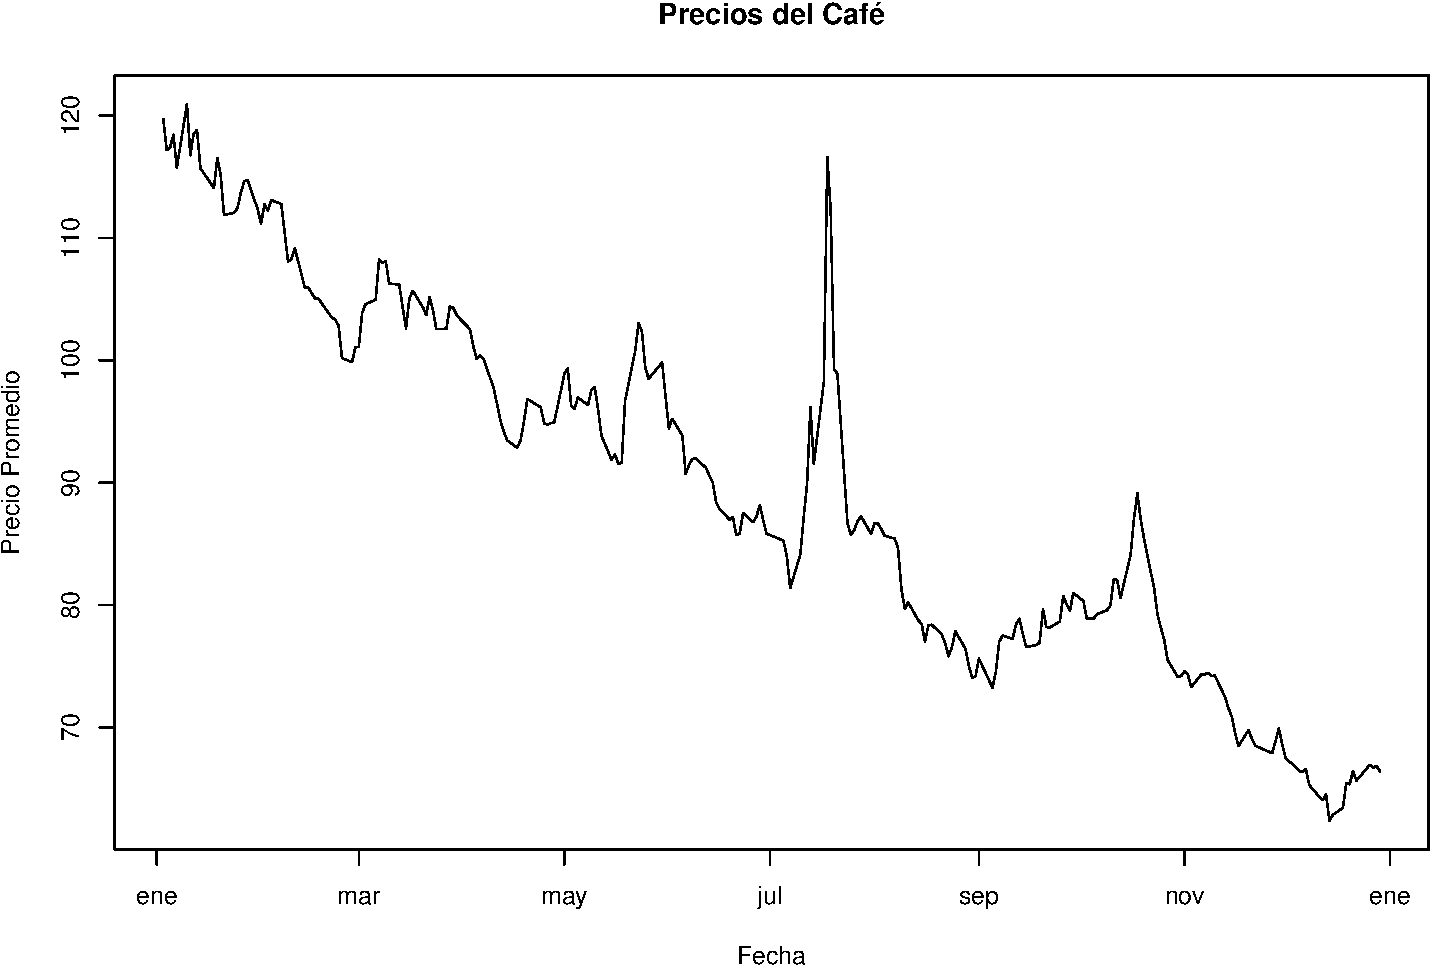
\includegraphics{Informe_files/figure-beamer/unnamed-chunk-4-1.pdf}
\end{frame}

\begin{frame}[fragile]{Serie de tiempo de todos los datos}
\phantomsection\label{serie-de-tiempo-de-todos-los-datos}
\begin{Shaded}
\begin{Highlighting}[]
\NormalTok{KCN4 }\OtherTok{\textless{}{-}} \FunctionTok{ts}\NormalTok{(datosHist}\SpecialCharTok{$}\NormalTok{precio\_promedio,}\AttributeTok{freq=}\DecValTok{12}\NormalTok{)}
\FunctionTok{plot}\NormalTok{(datosHist}\SpecialCharTok{$}\NormalTok{Fecha, KCN4, }\AttributeTok{type =} \StringTok{"l"}\NormalTok{, }\AttributeTok{xlab =} \StringTok{"Fecha"}\NormalTok{, }
     \AttributeTok{ylab =} \StringTok{"Precio Promedio"}\NormalTok{, }\AttributeTok{main =} \StringTok{"Precios del Café"}\NormalTok{)}
\end{Highlighting}
\end{Shaded}

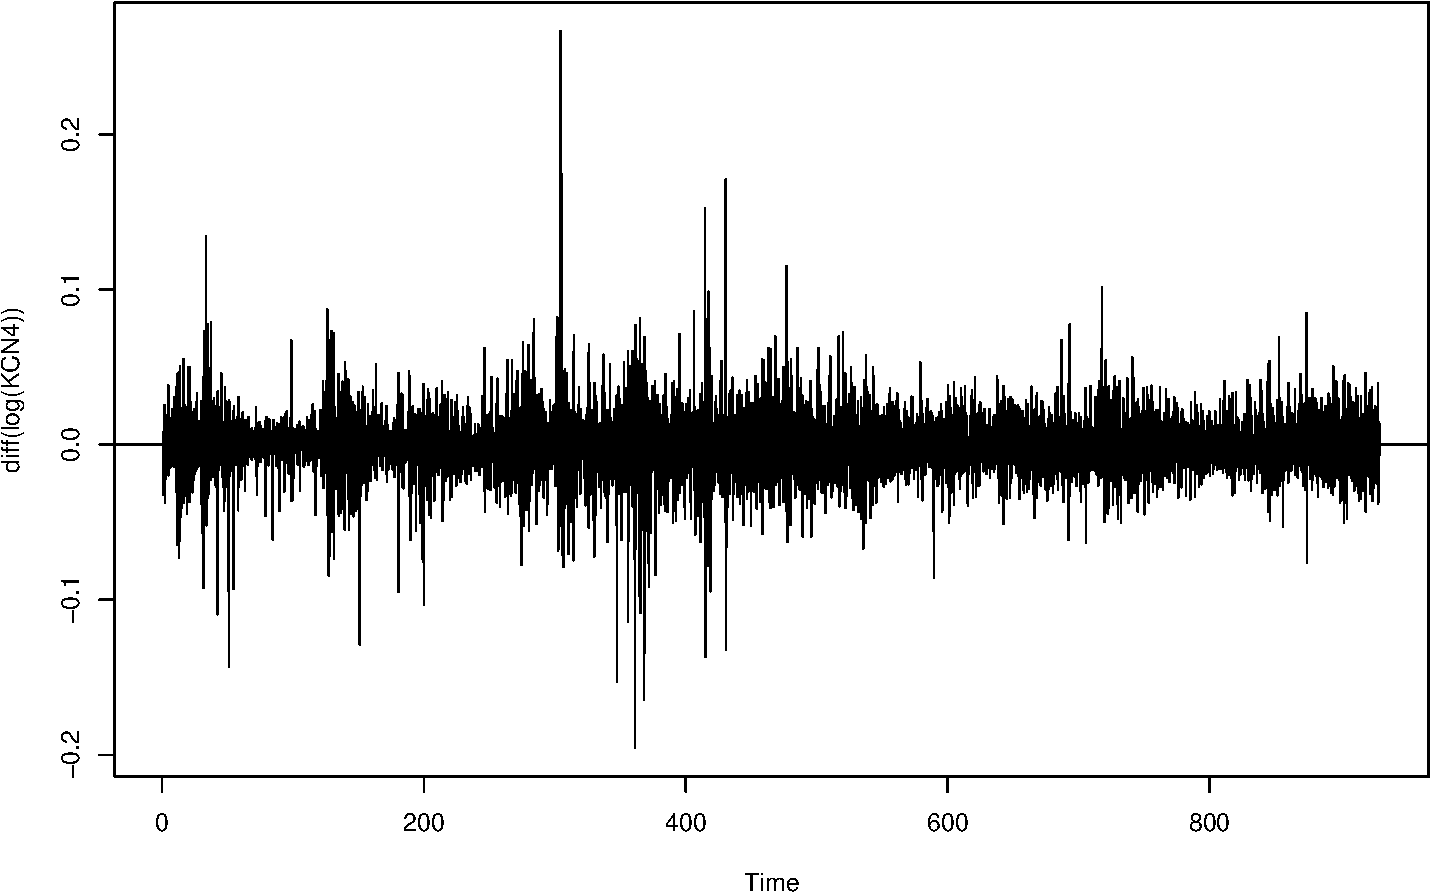
\includegraphics{Informe_files/figure-beamer/unnamed-chunk-5-1.pdf}
\end{frame}

\begin{frame}[fragile]{Serie de tiempo por año}
\phantomsection\label{serie-de-tiempo-por-auxf1o}
\begin{Shaded}
\begin{Highlighting}[]
\CommentTok{\# Crear un bucle for para particionar los datos por año}
\ControlFlowTok{for}\NormalTok{ (i }\ControlFlowTok{in} \DecValTok{1980}\SpecialCharTok{:}\DecValTok{2023}\NormalTok{) \{}
\NormalTok{  start\_date }\OtherTok{\textless{}{-}} \FunctionTok{as.Date}\NormalTok{(}\FunctionTok{paste}\NormalTok{(i, }\StringTok{"{-}01{-}01"}\NormalTok{, }\AttributeTok{sep =} \StringTok{""}\NormalTok{))}
\NormalTok{  end\_date }\OtherTok{\textless{}{-}} \FunctionTok{as.Date}\NormalTok{(}\FunctionTok{paste}\NormalTok{(i }\SpecialCharTok{+} \DecValTok{1}\NormalTok{, }\StringTok{"{-}01{-}01"}\NormalTok{, }\AttributeTok{sep =} \StringTok{""}\NormalTok{))}
  
\NormalTok{  datosporAño }\OtherTok{\textless{}{-}} \FunctionTok{subset}\NormalTok{(datosHist, }
\NormalTok{                        Fecha }\SpecialCharTok{\textgreater{}=}\NormalTok{ start\_date }
                        \SpecialCharTok{\&}\NormalTok{ Fecha }\SpecialCharTok{\textless{}}\NormalTok{ end\_date)}
\NormalTok{  KCN4porAño }\OtherTok{\textless{}{-}} \FunctionTok{ts}\NormalTok{(datosporAño}\SpecialCharTok{$}\NormalTok{precio\_promedio, }
                   \AttributeTok{frequency =} \DecValTok{12}\NormalTok{)}
  \FunctionTok{assign}\NormalTok{(}\FunctionTok{paste0}\NormalTok{(}\StringTok{"Datos\_Hist\_"}\NormalTok{, i), datosporAño)}
  \FunctionTok{assign}\NormalTok{(}\FunctionTok{paste0}\NormalTok{(}\StringTok{"KCN4\_"}\NormalTok{, i), KCN4porAño)}
\NormalTok{\}}
\end{Highlighting}
\end{Shaded}
\end{frame}

\begin{frame}[fragile]{}
\phantomsection\label{section}
\begin{Shaded}
\begin{Highlighting}[]
\FunctionTok{plot}\NormalTok{(Datos\_Hist\_2000}\SpecialCharTok{$}\NormalTok{Fecha, KCN4\_2000, }\AttributeTok{type =} \StringTok{"l"}\NormalTok{, }
     \AttributeTok{xlab =} \StringTok{"Fecha"}\NormalTok{, }
     \AttributeTok{ylab =} \StringTok{"Precio Promedio"}\NormalTok{, }\AttributeTok{main =} \StringTok{"Precios del Café"}\NormalTok{)}
\end{Highlighting}
\end{Shaded}

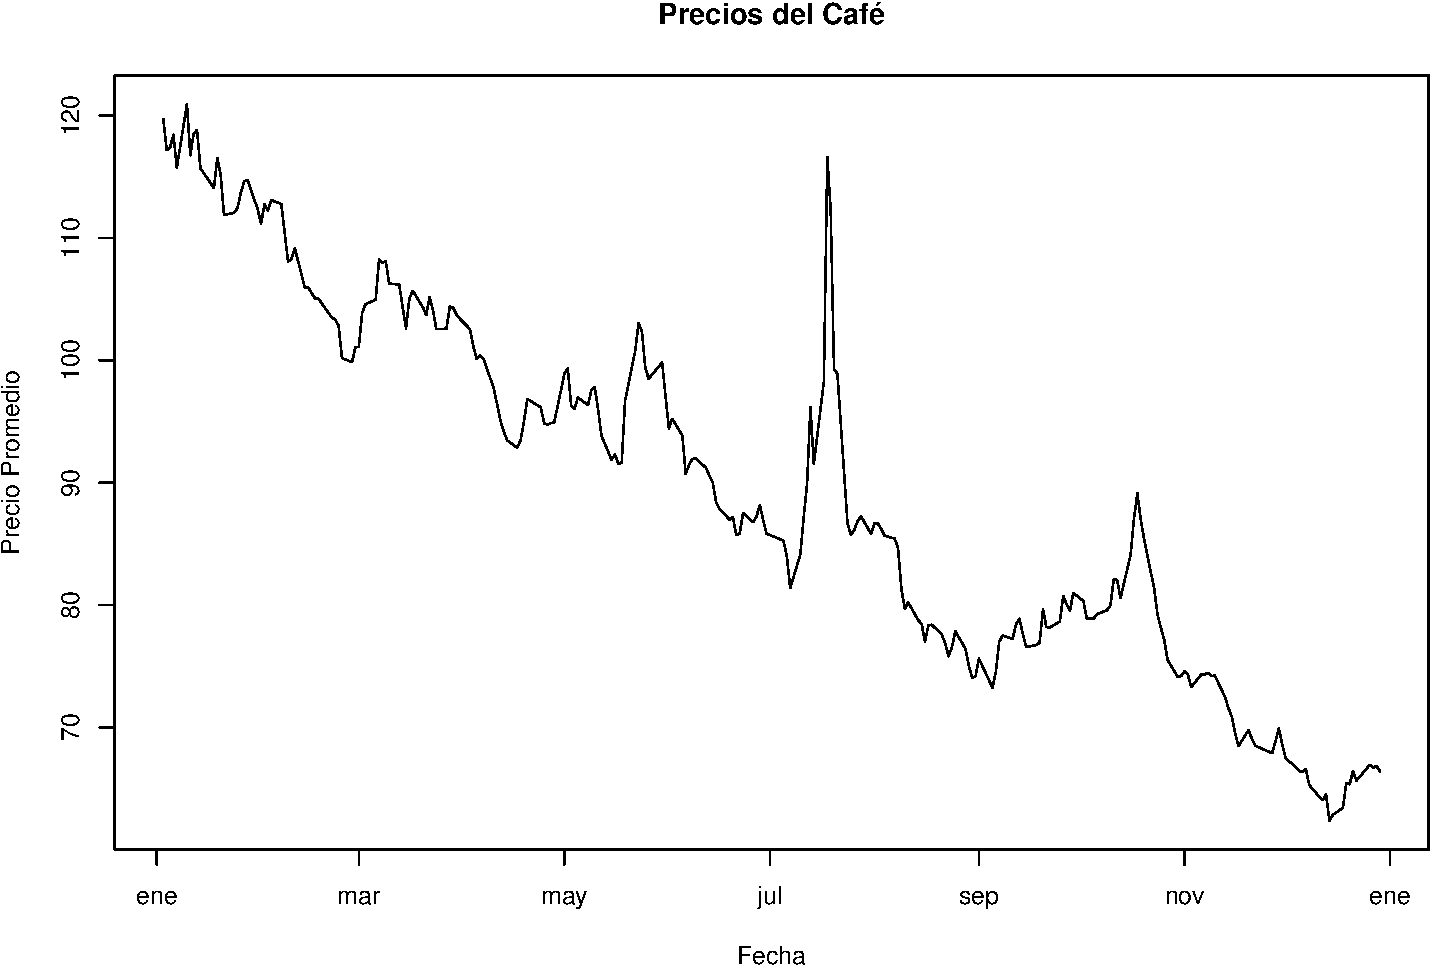
\includegraphics{Informe_files/figure-beamer/unnamed-chunk-7-1.pdf}
\end{frame}

\begin{frame}{Cálculo de la variación de las series de tiempo}
\phantomsection\label{cuxe1lculo-de-la-variaciuxf3n-de-las-series-de-tiempo}
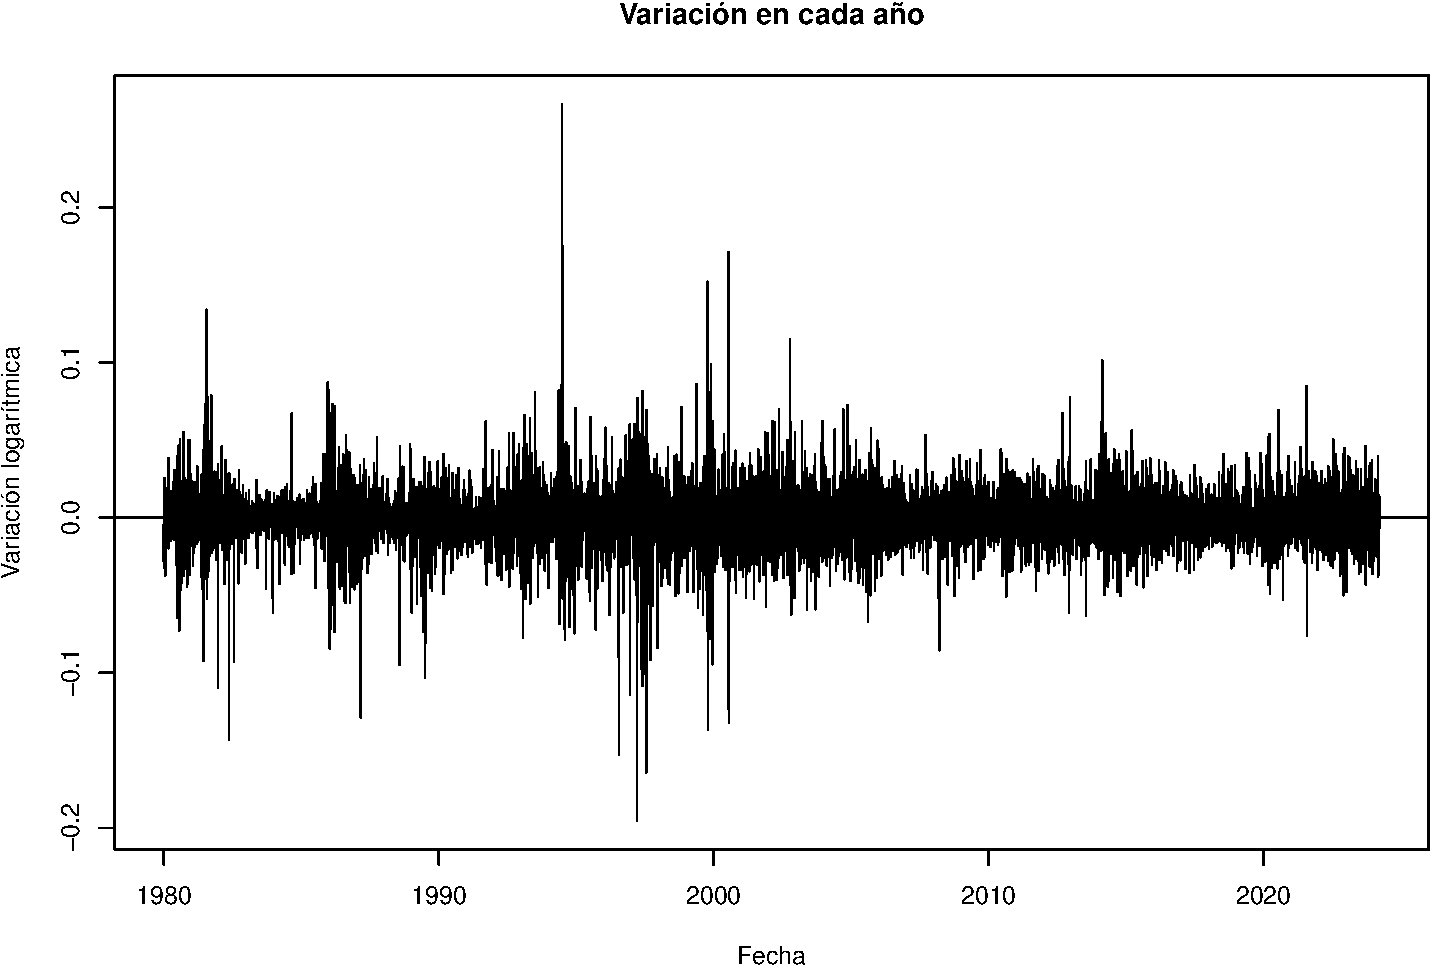
\includegraphics{Informe_files/figure-beamer/unnamed-chunk-8-1.pdf}
\end{frame}

\begin{frame}{}
\phantomsection\label{section-1}
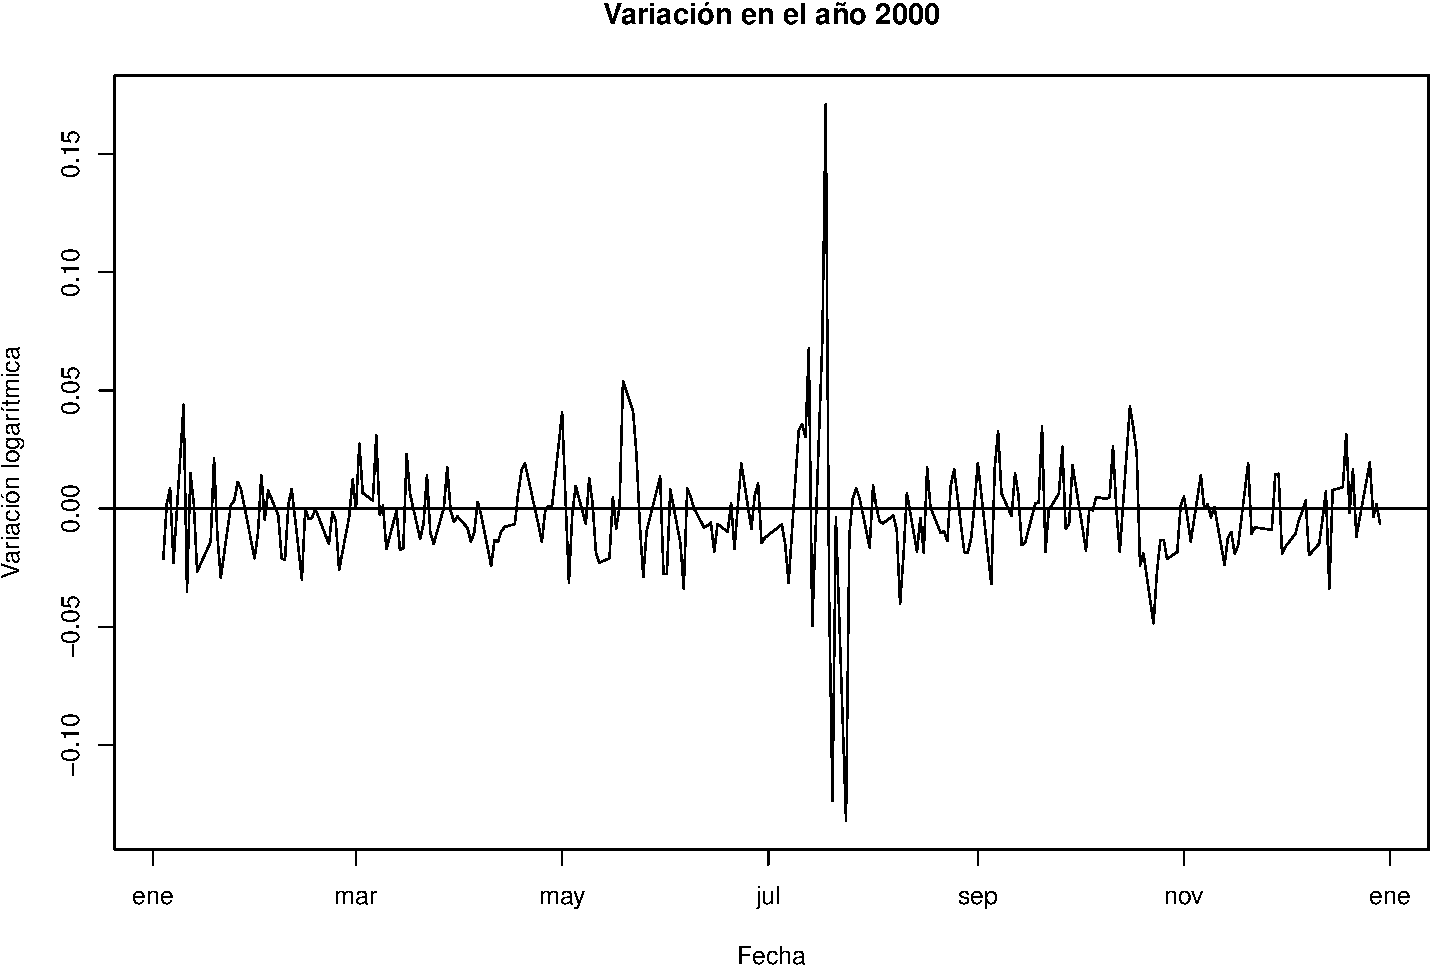
\includegraphics{Informe_files/figure-beamer/unnamed-chunk-9-1.pdf}
\end{frame}

\begin{frame}[fragile]{Descomposición de la serie de tiempo}
\phantomsection\label{descomposiciuxf3n-de-la-serie-de-tiempo}
\begin{Shaded}
\begin{Highlighting}[]
\NormalTok{decomposition\_2000 }\OtherTok{\textless{}{-}} \FunctionTok{decompose}\NormalTok{(KCN4\_2000, }
                                \AttributeTok{type =} \StringTok{"additive"}\NormalTok{)}
\FunctionTok{plot}\NormalTok{(decomposition\_2000}\SpecialCharTok{$}\NormalTok{x, }
     \AttributeTok{ylab =} \StringTok{"Serie de Tiempo Original"}\NormalTok{, }\AttributeTok{xlab =} \StringTok{""}\NormalTok{)}
\end{Highlighting}
\end{Shaded}

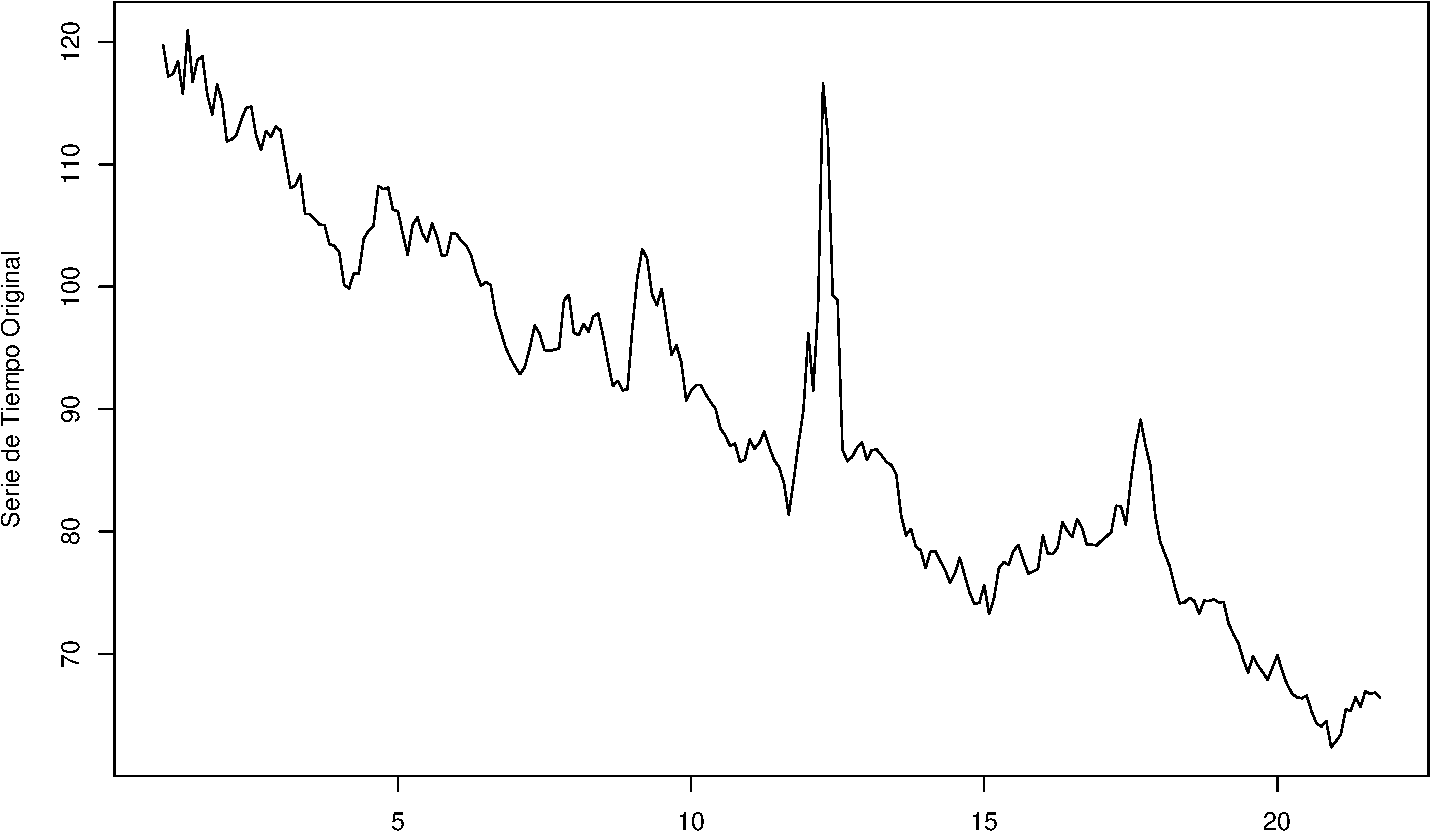
\includegraphics{Informe_files/figure-beamer/unnamed-chunk-10-1.pdf}
\end{frame}

\begin{frame}[fragile]{}
\phantomsection\label{section-2}
\begin{Shaded}
\begin{Highlighting}[]
\FunctionTok{plot}\NormalTok{(decomposition\_2000}\SpecialCharTok{$}\NormalTok{trend, }
     \AttributeTok{ylab =} \StringTok{"Tendencia"}\NormalTok{, }\AttributeTok{xlab =} \StringTok{""}\NormalTok{)}
\end{Highlighting}
\end{Shaded}

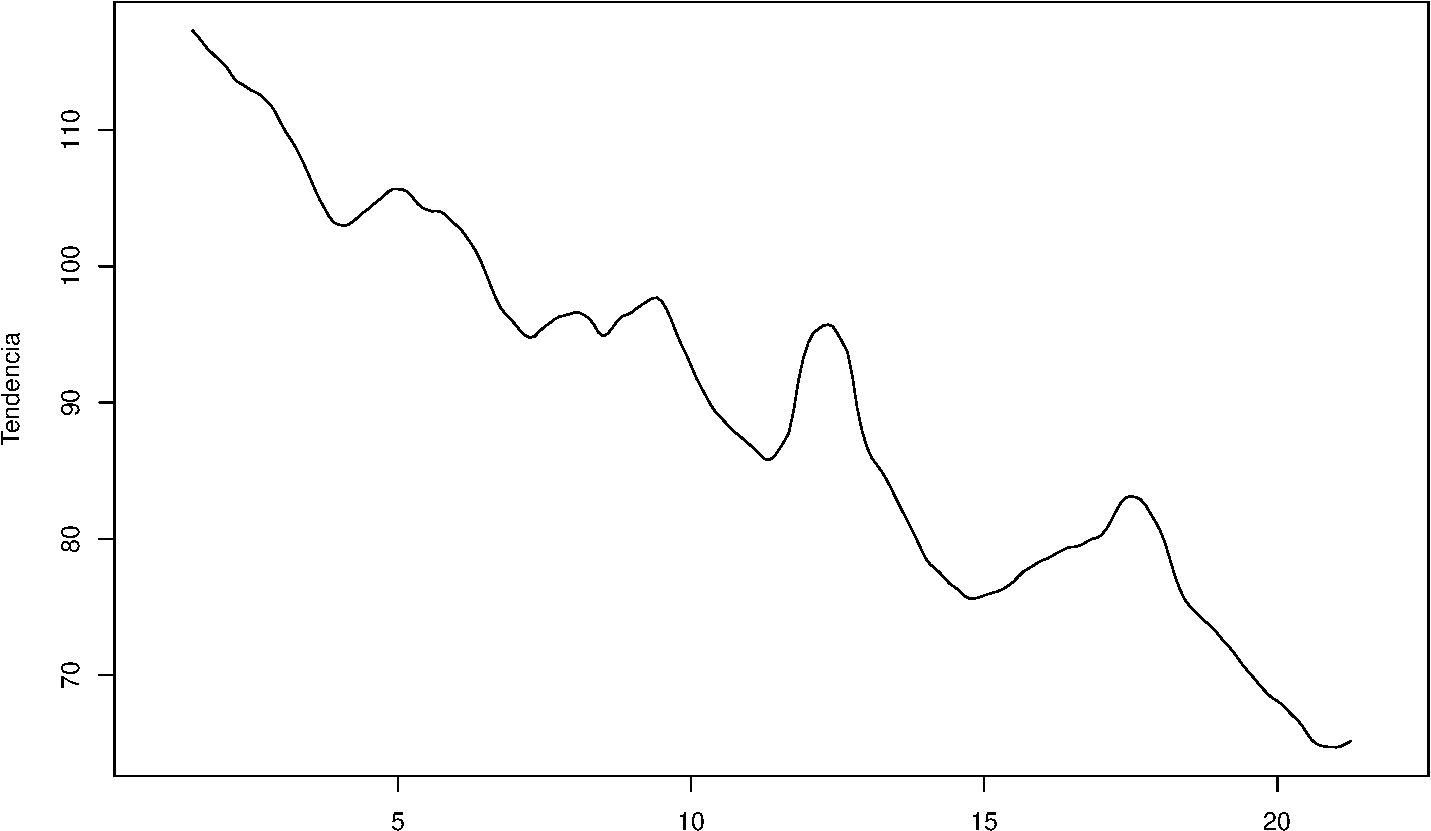
\includegraphics{Informe_files/figure-beamer/unnamed-chunk-11-1.pdf}
\end{frame}

\begin{frame}[fragile]{}
\phantomsection\label{section-3}
\begin{Shaded}
\begin{Highlighting}[]
\FunctionTok{plot}\NormalTok{(decomposition\_2000}\SpecialCharTok{$}\NormalTok{seasonal, }
     \AttributeTok{ylab =} \StringTok{"Estacionalidad"}\NormalTok{, }\AttributeTok{xlab =} \StringTok{""}\NormalTok{)}
\end{Highlighting}
\end{Shaded}

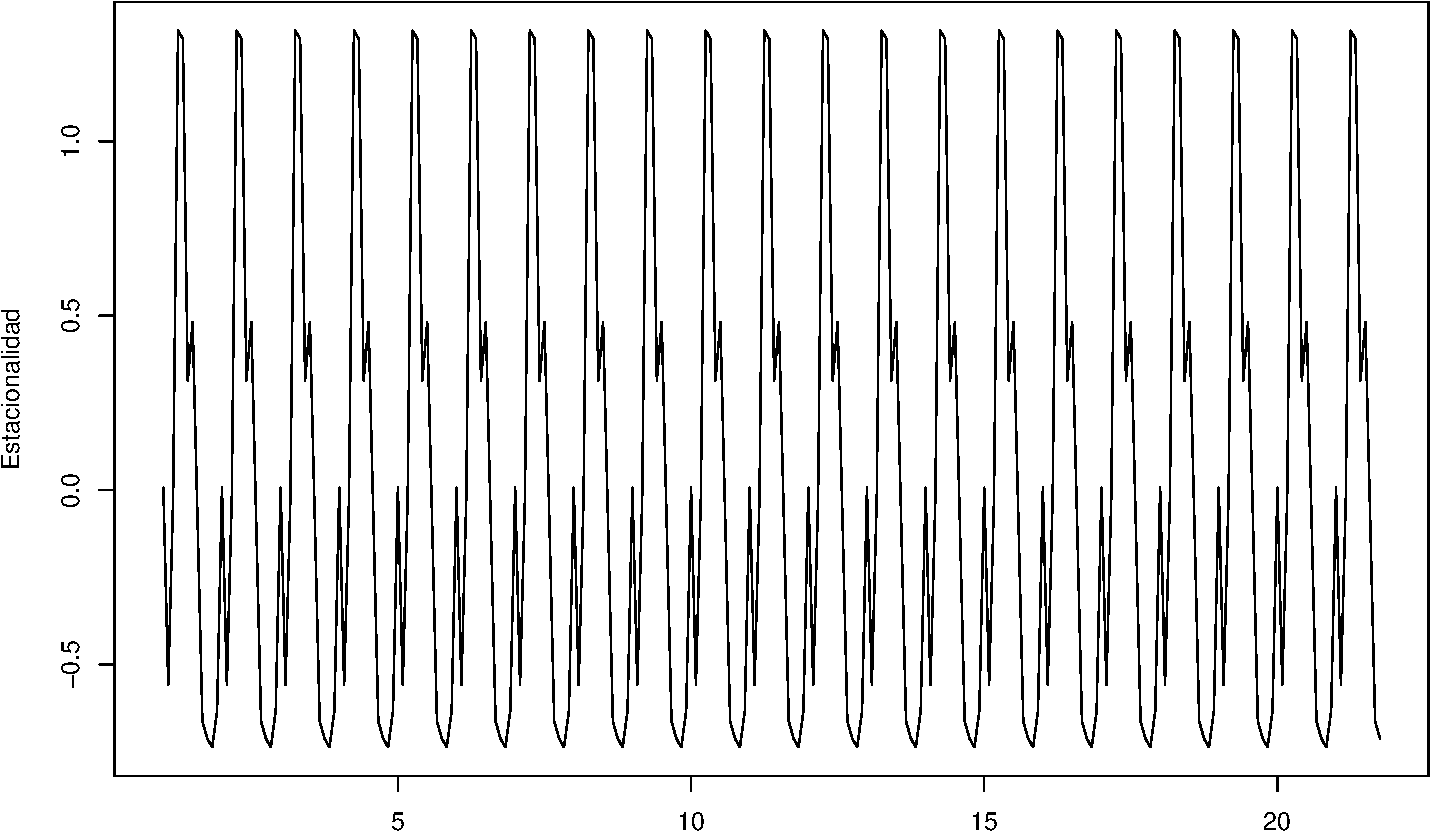
\includegraphics{Informe_files/figure-beamer/unnamed-chunk-12-1.pdf}
\end{frame}

\begin{frame}[fragile]{}
\phantomsection\label{section-4}
\begin{Shaded}
\begin{Highlighting}[]
\FunctionTok{plot}\NormalTok{(decomposition\_2000}\SpecialCharTok{$}\NormalTok{random, }
     \AttributeTok{ylab =} \StringTok{"Residuales"}\NormalTok{, }\AttributeTok{xlab =} \StringTok{""}\NormalTok{)}
\end{Highlighting}
\end{Shaded}

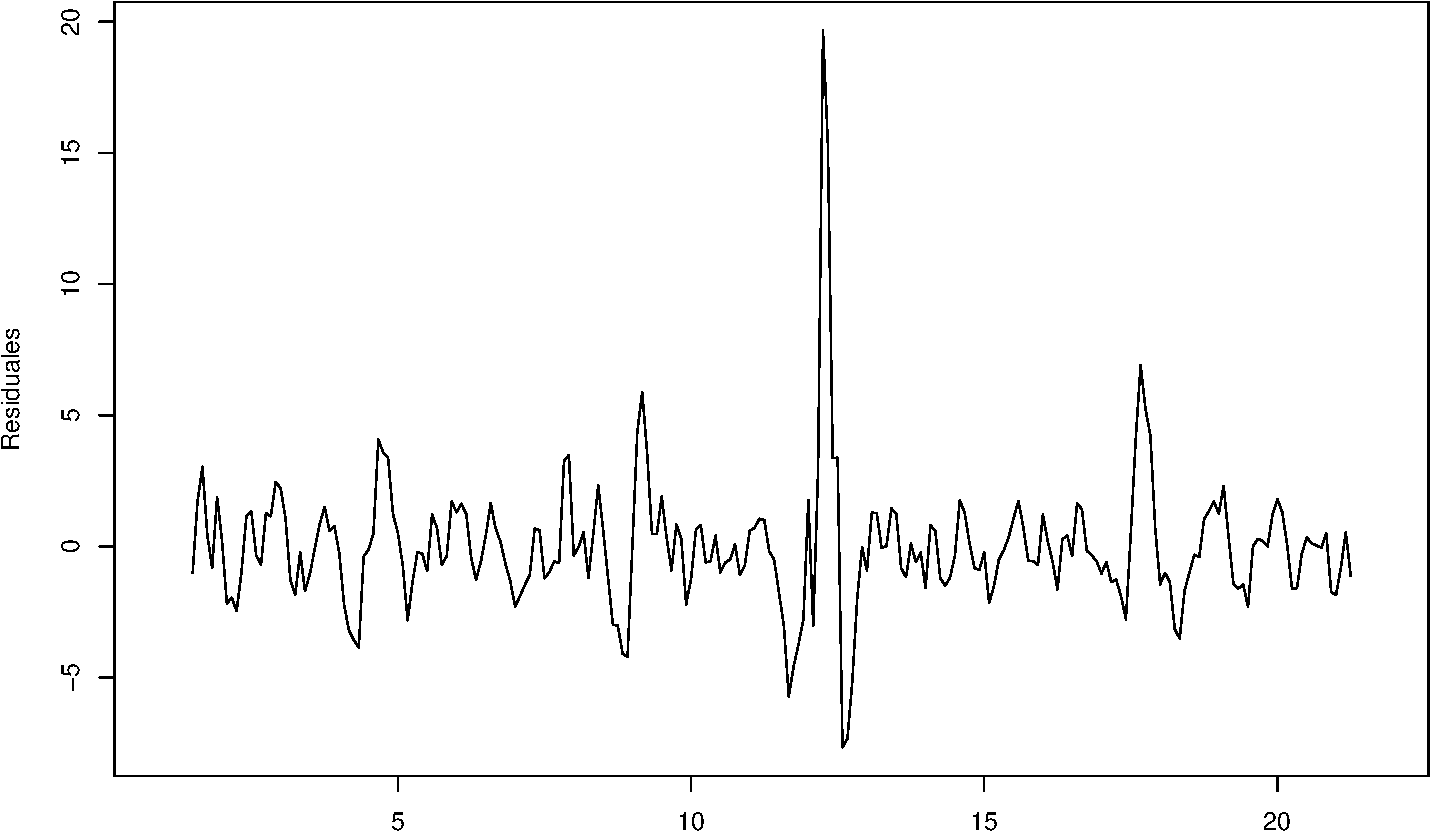
\includegraphics{Informe_files/figure-beamer/unnamed-chunk-13-1.pdf}
\end{frame}

\begin{frame}[fragile]{Análisis de tendencia}
\phantomsection\label{anuxe1lisis-de-tendencia}
\begin{Shaded}
\begin{Highlighting}[]
\FunctionTok{plot}\NormalTok{(decomposition\_2000}\SpecialCharTok{$}\NormalTok{x, }
     \AttributeTok{ylab =} \StringTok{"Serie de Tiempo Original"}\NormalTok{, }\AttributeTok{xlab =} \StringTok{""}\NormalTok{)}
\FunctionTok{abline}\NormalTok{(}\FunctionTok{lm}\NormalTok{(decomposition\_2000}\SpecialCharTok{$}\NormalTok{x }
          \SpecialCharTok{\textasciitilde{}} \FunctionTok{time}\NormalTok{(decomposition\_2000}\SpecialCharTok{$}\NormalTok{x)), }\AttributeTok{col =} \StringTok{"red"}\NormalTok{)}
\end{Highlighting}
\end{Shaded}

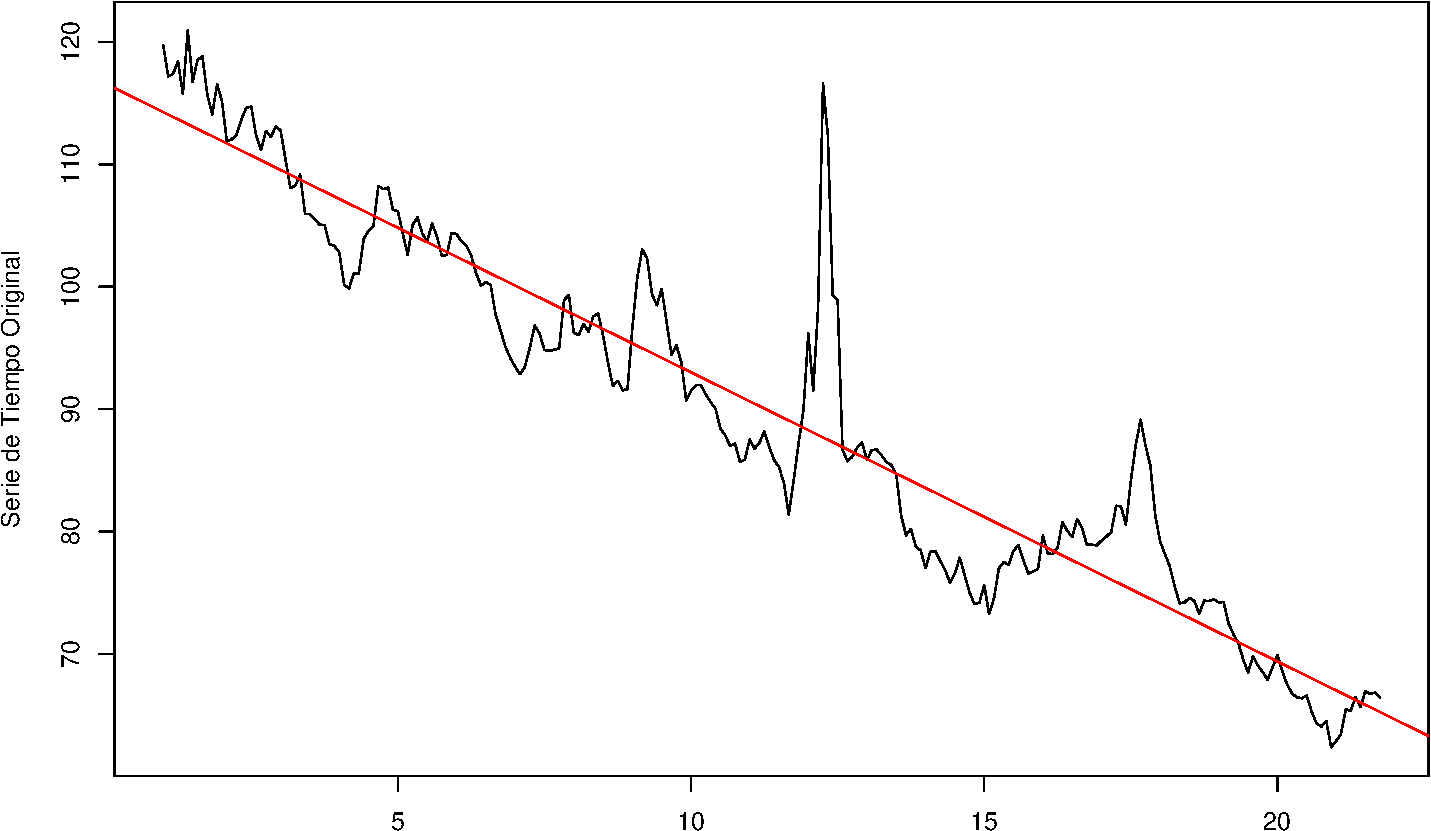
\includegraphics{Informe_files/figure-beamer/unnamed-chunk-14-1.pdf}
\end{frame}

\begin{frame}[fragile]{}
\phantomsection\label{section-5}
\begin{Shaded}
\begin{Highlighting}[]
\FunctionTok{plot}\NormalTok{(decomposition\_2000}\SpecialCharTok{$}\NormalTok{trend, }
     \AttributeTok{ylab =} \StringTok{"Tendencia"}\NormalTok{, }\AttributeTok{xlab =} \StringTok{""}\NormalTok{)}
\end{Highlighting}
\end{Shaded}

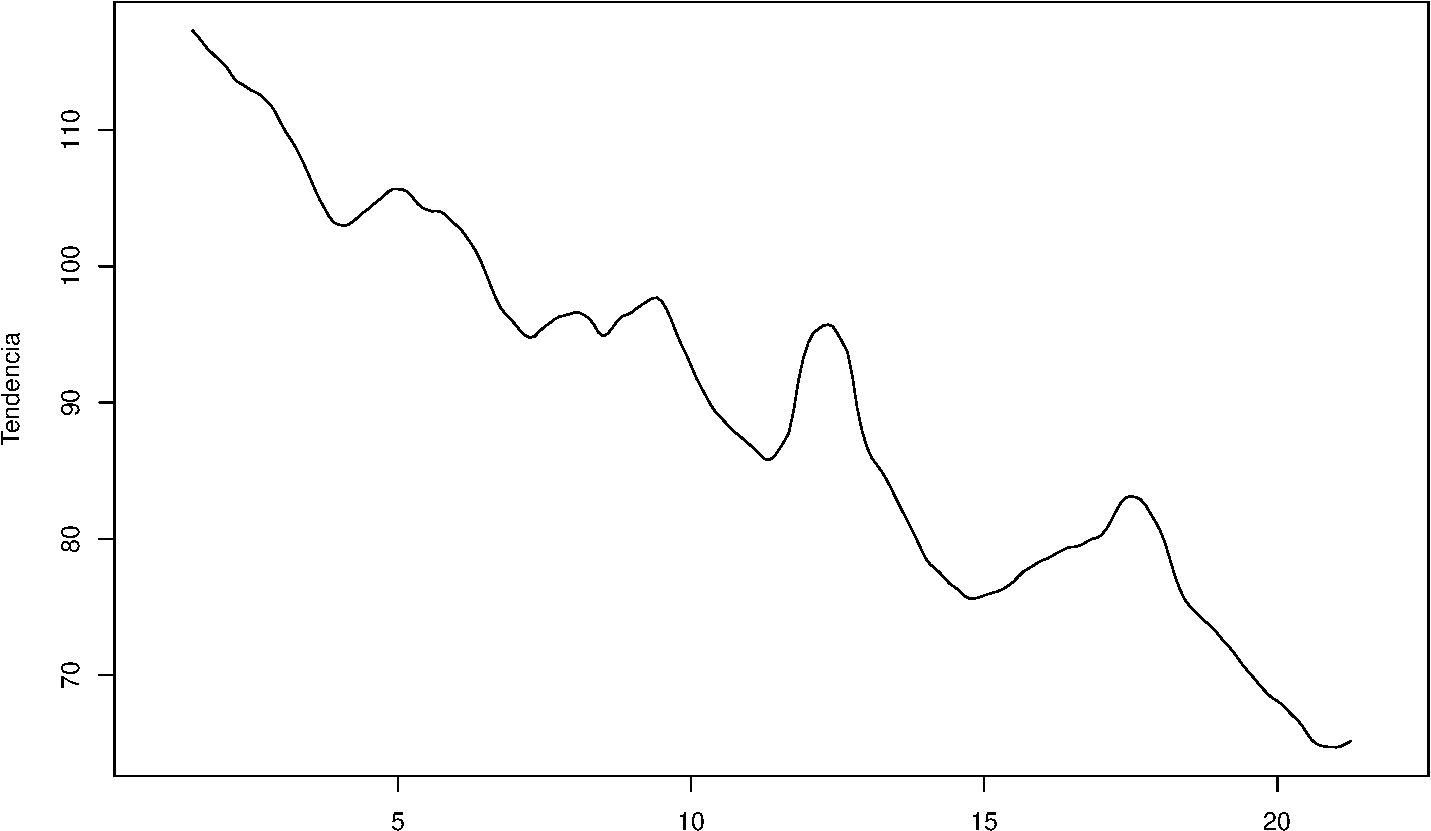
\includegraphics{Informe_files/figure-beamer/unnamed-chunk-15-1.pdf}
\end{frame}

\begin{frame}[fragile]{Estacionariedad}
\phantomsection\label{estacionariedad}
\[H_0: \text{No es estacionaria.}\] \[H_1: \text{Es estacionaria}\]

\begin{verbatim}
##                                                    Resumen
## 1  F-statistic: 8.203 on 3 and 244 DF,  p-value: 3.185e-05
## 2                                                         
## 3                                                         
## 4      Value of test-statistic is: -4.6517 7.7753 10.8352 
## 5                                                         
## 6                    Critical values for test statistics: 
## 7                                         1pct  5pct 10pct
## 8                                   tau3 -3.99 -3.43 -3.13
## 9                                   phi2  6.22  4.75  4.07
## 10                                  phi3  8.43  6.49  5.47
## 11
\end{verbatim}
\end{frame}

\begin{frame}{Conclusión}
\phantomsection\label{conclusiuxf3n}
Basado en el resumen del test de Dickey-Fuller aumentado (ADF) para
verificar la estacionariedad de la serie de tiempo de los precios del
café (KCN4\_2000)

\textbf{Planteamiento de la Hipótesis del Test de Dickey-Fuller:}

-Hipótesis Nula (H0): La serie de tiempo NO es estacionaria.

-Hipótesis Alternativa (H1): La serie de tiempo es estacionaria.

\textbf{Resultado del Test}

El valor p obtenido del test de Dickey-Fuller Aumentado es 3.185e-05,
que es significativamente menor que cualquier nivel de significancia
comúnmente utilizado (como 1\%, 5\% o 10\%). Esto indica una fuerte
evidencia en contra de la hipótesis nula (H0) de que la serie de tiempo
es estacionaria.

Esta conclusión sirve para el análisis y la predicción de los precios
del café, ya que una serie estacionaria permite utilizar modelos
adecuados de series temporales, como los modelos ARIMA, para realizar
pronósticos más precisos y confiables.
\end{frame}

\begin{frame}{Referencias}
\phantomsection\label{referencias}
\begin{itemize}
\item
  Walpole, R. E., Myers, R. H., Myers, S. L., \& Ye, K. (2020).
  Probabilidad y estadística para ingeniería y ciencias (9.a ed., L. E.
  Pineda Ayala, Trad.). Pearson.
\item
  Wackerly, D. D., Mendenhall III, W., \& Scheaffer, R. L. (2010).
  Estadística matemática con aplicaciones (7.a ed., J. H. Romo Muñoz,
  Trad.). Cengage Learning.
\item
  Brockwell, P. J., \& Davis, R. A. (2002). Introduction to Time Series
  and Forecasting (2nd ed.). Springer.
\end{itemize}
\end{frame}

\end{document}
